\documentclass[12pt]{article}
\title{\LaTeX}
\date{}

\title{\emph{\huge\textbf{Start up Guide \\ for \\$n^3He$ Analysis}}
}
\author{\\Latiful Kabir\\
}

\usepackage{listings}
\usepackage{color}
\usepackage{hyperref}
\usepackage{graphicx}

\definecolor{dkgreen}{rgb}{0,0.6,0}
\definecolor{gray}{rgb}{0.5,0.5,0.5}
\definecolor{mauve}{rgb}{0.58,0,0.82}

\lstset{frame=tb,
  language=C,
  aboveskip=3mm,
  belowskip=3mm,
  showstringspaces=false,
  columns=flexible,
  basicstyle={\small\ttfamily},
  numbers=none,
  numberstyle=\tiny\color{gray},
  keywordstyle=\color{blue},
  commentstyle=\color{dkgreen},
  stringstyle=\color{mauve},
  breaklines=true,
  breakatwhitespace=true,
  tabsize=3
}

\begin{document}
  \maketitle
  
\newpage  
\tableofcontents
\newpage
\setcounter{tocdepth}{2}

\section{Resources}
All the start up software and manual related to $n^3He$ experiment can be found from the official git repository with detailed instruction. \\
The easiest way is to go to n3He wiki (n3he.wikispaces.com) and then click on software from the left panel.  \\
Alternatively, here is a direct \href{http://latifkabir.github.io/n3He_Soft/}{link}.\\
Any new change goes to this  git repository. You might want to clone the entire repository and pull periodically to be updated. Or you can also download the last release of only what your are interested in.  

\noindent
{\color{red} \rule{\linewidth}{1mm} }
 
\newpage
\section{Quick start on basestar}
On basestar the data is being transferred and saved to the directory \\ \textcolor{magenta}{ /mnt/idata01/data/ }and the analysis library is compiled in a shared directory \textcolor{magenta}{ /home/npdg/n3He/libn3He/lib} 

So a quick start using the compiled library can be as follows from any user account:

\begin{enumerate}
  \item Add the following lines to the .bashrc file \& save it
 
\begin{lstlisting}
if [ -f /home/npdg/n3He/libn3He/bin/thisn3He.sh ]; then
       . /home/npdg/n3He/libn3He/bin/thisn3He.sh
fi
\end{lstlisting}

 \item Start a new terminal , go to  \textcolor{magenta} { /home/npdg/n3He/libn3He/analysis/ }directory \& try running sample analysis scripts from ROOT.
 \item The data browser GUI (named as n3HeData) can be opened issuing the command\textcolor{magenta}{ /home/npdg/n3He/n3HeData/n3HeData } from the terminal. Copy the binary to your home directory if you will be using the GUI frequently.
\end{enumerate}

Other user specific customization can be achieved following the instruction in the ReadMe file in the respective directory.\\
For a local version of the library and data browser please read the corresponding section.

\noindent
{\color{red} \rule{\linewidth}{1mm} }
 
\newpage
\section{Event length and file size calculation}
The  event length set in the clean DAQ at 50 KHz sample rate is :830 . Theoretically the maximum possible value is 50KHz x 16.66 ms = 833 samples per T0 . \\
But 833 event length gives occasional overlap. So we set to 830. \\
For dirty DAQ at 100 KHz the theoretical number of samples 100KHz x 16.66 ms = 1666 \\
But to avoid overlap we set to 1660. \\
More over the DAQ has fixed dead time(readout time) of 35 samples(with no averaging) at the end of any event. This amount of time will be missed for every event.\\
\\
Clean DAQ event length 830 with nacc=16,16 with hi resolution mode=1\\
Dirty DAQ event length 1660 with nacc=1,1 with hi resolution mode=0\\
where nacc=n,n indicates how many samples being averaged.\\
\\
Thus number of sample per event:\\
Clean DAQ: (830-35)/16=49.68 $\sim$ 50  (1 header + 49 samples)\\
Dirty DAQ: (1660-35)=1625 (1 header + 1624 samples) \\
\\
Run Length calculation:\\
With 25000 T0 per run: \\
Clean DAQ file size: 25000 T0 x 50 samples x 4 Byte per sample x 48 Channels =$240 \times 10^6$ Bytes\\
Dirty DAQ file size (before process): 25000 T0 x 1625 samples x 4 Bytes per sample x 8 channels = $1300 \times 10^6$ Bytes\\
Dirty DAQ file seize (after process) : 25000 T0 x 1625 samples x 4 Bytes per sample x 2 channels = $325 \times 10^6$ Bytes\\
\noindent
{\color{red} \rule{\linewidth}{1mm} }
 
\newpage
\section{The data file structure}
48 Clean DAQ channels divided into two modules: \\
Each sample is 4 bytes(in hexdump one contiguous pair consists one sample or 4 bytes).\\
\begin{figure}[htb]
\centering
% Requires \usepackage{graphicx}
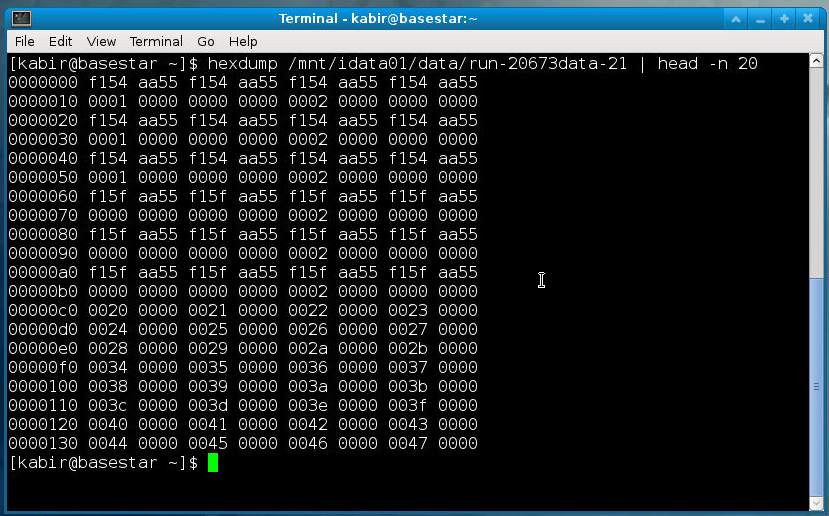
\includegraphics[width=6in]{hexdump.png}\\
\caption{Typical view of hexdump}\label{f1}
\end{figure}
The above hexdump to be interpreted as follows:\\
With: mod= module  ch = channel\\
\begingroup
    \fontsize{8pt}{12pt}\selectfont
    \begin{verbatim}      
mod1event1sample1Ch0 mod1event1sample1ch1 mod1event1sample1ch3 ..... ... ... ... ... mod1event1sample1ch8 
mod1event1sample1Ch9 mod1event1sample1ch10 mod1event1sample1ch11 ..... ... ... ... ... mod1event1sample1ch16
mod1event1sample1Ch17 mod1event1sample1ch18 mod1event1sample1ch19 ..... ... ... ... ... mod1event1sample1ch23

mod2event1sample1Ch0 mod2event1sample1ch1 mod2event1sample1ch3 ..... ... ... ... ... mod2event1sample1ch8 
mod2event1sample1Ch9 mod2event1sample1ch10 mod2event1sample1ch11 ..... ... ... ... ... mod2event1sample1ch16
mod2event1sample1Ch17 mod2event1sample1ch18 mod2event1sample1ch19 ..... ... ... ... ... mod2event1sample1ch23


mod1event2sample1Ch0 mod1event2sample1ch1 mod1event2sample1ch3 ..... ... ... ... ... mod1event2sample1ch8 
mod1event2sample1Ch9 mod1event2sample1ch10 mod1event2sample1ch11 ..... ... ... ... ... mod1event2sample1ch16
mod1event2sample1Ch17 mod1event2sample1ch18 mod1event2sample1ch19 ..... ... ... ... ... mod1event2sample1ch23

mod2event2sample1Ch0 mod2event2sample1ch1 mod2event2sample1ch3 ..... ... ... ... ... mod2event2sample1ch8
mod2event2sample1Ch9 mod2event2sample1ch10 mod2event2sample1ch11 ..... ... ... ... ... mod2event2sample1ch16
mod2event2sample1Ch17 mod2event2sample1ch18 mod2event2sample1ch19 ..... ... ... ... ... mod2event2sample1ch23
  
....     ....             ....  ...           .................             ........................    .....
....     ....             ....  ...           .................             ........................    .....
....     ....             ....  ...           .................             ........................    .....
....     ....             ....  ...           .................             ........................    .....

Up to N number of events.
\end{verbatim}    
\endgroup

Now the first sample of any event is the event header with following structure:\\
mod1event1sample1Ch0=mod1event1sample1Ch1=mod1event1sample1Ch3 = Event Signature-1 (0xaa55f154) ,\\ mod1event1sample1Ch4= Event Number\\
mod1event1sample1Ch5 = checksum using path-1  \\mod1event1sample1Ch6 = sample number \\mod1event1sample1Ch7 = checksum using path-2 \\
Then this pattern repeats 3 more times (i.e. in quanta of 8 channels) up to channel-23\\
\\
mod2event1sample1Ch0 =mod2event1sample1Ch1 = mod2event1sample1Ch3= Event Signature-2 (0xaa55f15f) \\mod1event1sample1Ch4= 0 (always)\\
mod2event1sample1Ch5 = checksum using path-1 \\ mod2event1sample1Ch6 = sample number \\mod2event1sample1Ch7 = checksum using path-2 \\
Then this pattern repeats 3 more times (i.e. in quanta of 8 channels) up to channel-23\\
\\
For Dirty DAQ the data is taken in 8 channels (bank mask B) with one module only and then processed to 2 channels.
On Batch panel, M1 signal is connected to marked channel-26 and RFSF signal is connected to marked channel 27. This corresponds to 
ADC channel-5 (with checksum) and channel-6 (with sample number) where for ADC channel number starts with 0.\\
\\
This for Dirty DAQ after the processing,\\
\\
event1sample1Ch0   event1sample1ch1\\
event2sample1Ch0   event2sample1ch1\\
... ... ... ... ... ... .........\\
.....  .........  ..... .... ....\\
\\
Up to N events.\\
\\
with the first sample of any event being checksum and sample number i.e.\\
     event1sample1ch0 = checksum.\\
     event1sample1ch1 = sample number.\\

\noindent
{\color{red} \rule{\linewidth}{1mm} }
 
\newpage
\section{The ADC channel to wire map}
Eventually the ADC channel to detector wire map to be handled by the library. However following is the map for reference:
\begin{lstlisting}

Number of layers = 16;
Number of wires per layer= 9;

Layer_to_DAQ_map[Nlayers]={21, 23, 21, 23, 21, 23, 21, 23,
                         22, 24, 22, 24, 22, 24, 22, 24};

Layer_to_ADC_channel_map[16][9] =
    {
      {0,1,2,3,4,5,6,7,8},
      {0,1,2,3,4,5,6,7,8},
      {9,10,11,12,13,14,15,16,17},
      {9,10,11,12,13,14,15,16,17},
      {24,25,26,27,28,29,30,31,32},
      {24,25,26,27,28,29,30,31,32},
      {33,34,35,36,37,38,39,40,41},
      {33,34,35,36,37,38,39,40,41},
      {0,1,2,3,4,5,6,7,8},
      {0,1,2,3,4,5,6,7,8},
      {9,10,11,12,13,14,15,16,17},
      {9,10,11,12,13,14,15,16,17},
      {24,25,26,27,28,29,30,31,32},
      {24,25,26,27,28,29,30,31,32},
      {33,34,35,36,37,38,39,40,41},
      {33,34,35,36,37,38,39,40,41},
    };
\end{lstlisting}

\noindent
{\color{red} \rule{\linewidth}{1mm} }
 
\newpage
\section{Setting up local version of n3He analysis library on basestar}
Eventually you will want to set up your own version of the analysis library and ROOT environment. This way you can modify any
part of the library and add more functionality. 

\begin{enumerate}
\item Download the source code from \href{http://latifkabir.github.io/n3He_Soft/}{here}. \\
lib3He is the analysis library for n3He experiment.

\item Make any necessary changes in Constants.h file that is required.

\item Do \textcolor{magenta}{ make} to compile the library. 

\item This will produce  \textcolor{magenta}{libn3He.so} (shared library will be inside lib directory).

\item Place the .so file in a directory under \textcolor{magenta}{ LD\_LIBRARY\_PATH }.

\item Now start root and load the Library as: \textcolor{magenta}{gSystem$->$Load(``libTree'')}  \& \textcolor{magenta}{gSystem$->$Load(``libn3He.so'')}  . (For Online analysis)

\item  For analysis from a script if you include TTree.h file then you need not to do \textcolor{magenta}{gSystem$->$Load(``libTree'')}; Just load 
    \textcolor{magenta}{gSystem$->$Load(``libn3He.so'')}.  You need to give full path unless the directory is included in \textcolor{magenta}{LD\_LIBRARY\_PATH}.

\item If you put the \textcolor{magenta}{rootlogon.C} file in \textcolor{magenta}{ macros } directory under Root installation directory, then the library will be loaded automatically and step-4 is NOT necessary.

\item Now from your root script create a Tree by calling: \textcolor{magenta}{TTreeRaw ${\ast}my\_tree$ = new TreeRaw(runNumber\#)} or Just \textcolor{magenta}{TTreeRaw t(runNumber\#)}

\item Do \textcolor{magenta}{$my\_tree->Print()$} to print the tree and branch structure.

\item Now do what ever analysis you want using \textcolor{magenta}{my\_tree }.

\item Try running example analysis scripts in ``analysis" directory.

\item To make life easier it's convenient to put the following command into your \textcolor{magenta}{$\sim$/.bash\_profile} or \textcolor{magenta}{$\sim$/.bashrc} file:

 
\begin{lstlisting}
if [ -f /path/to/libn3He/bin/thisn3He.sh ]; then 
        . /path/to/libn3He/bin/thisn3He.sh
 fi 
\end{lstlisting}

Note: This version of the library works both for ROOT 5 and ROOT 6.

\end{enumerate}

\noindent
{\color{red} \rule{\linewidth}{1mm} }
 
\newpage
\section{Setting up local version of data browser on basestar}
\begin{enumerate}
\item Download the source code from \href{http://latifkabir.github.io/n3He_Soft/}{here}. \\

\item In bin directory: contains just binary files(obtained after doing make) named \textcolor{magenta}{n3HeData}.

\item In libn3He directory: Contains all the library required for running the Data check GUI.

\item Modify and compile the library:(Unless you have already set up the library)
   You need to change the Data file directory from \textcolor{magenta}{Constants.h} in \textcolor{magenta}{libn3He} to appropriate directory. Before you do \textcolor{magenta}{make} do: \textcolor{magenta}{make clean}   
   in the same directory.  and then make a fresh shared binary files after you make any changes.

\item Place .so file under \textcolor{magenta}{LD\_LIBRARY\_PATH}:
   Now make sure the shared library (\textcolor{magenta}{libn3He.so}) file is in a directory under your \textcolor{magenta}{LD\_LIBRARY\_PATH}. 

   OR, a more professional way is as follows:
   Open \textcolor{magenta}{\*/libn3He/bin/thisn3He.sh} and define \textcolor{magenta}{n3HeROOT} path variable to the location where \textcolor{magenta}{libn3He} is located.
   for example: \textcolor{magenta}{n3HeROOT=/home/siplu/libn3He/}
   
   Now include command in your \textcolor{magenta}{.bashrc} file to run \textcolor{magenta}{thisn3He.sh} file each time you open the terminal. i.e. include the following lines:

\begin{lstlisting}
if [ -f path_to/libn3He/bin/thisn3He.sh ]; then
	. path_to/libn3He/bin/thisn3He.sh
fi
\end{lstlisting}

\item Produce binary for GUI:
  To produce a new binary file named \textcolor{magenta}{n3HeData}, go to n3HeData directory, open makefile and change \textcolor{magenta}{LIB\_INCLUDE} and \textcolor{magenta}{GLIBS} to
  appropriate location for you and then do \textcolor{magenta}{make}. It will produce \textcolor{magenta}{n3HeData} binary file in the same directory. 

\item Run the GUI:
 Now run the binary file \textcolor{magenta}{n3HeData} by doing \textcolor{magenta}{./n3HeData} from your recently compiled verson in \textcolor{magenta}{\*/n3He\_DAQ\_GUI/n3HeData/} .

\item Modify the \textcolor{magenta}{.desktop} file (included one only for Ubuntu distribution) and \textcolor{magenta}{.sh} file in bin directory accordingly and place it in your desktop if you want to run the GUI just by double clicking from your desktop.

\end{enumerate}

\begin{figure}[htb]
\centering
% Requires \usepackage{graphicx}
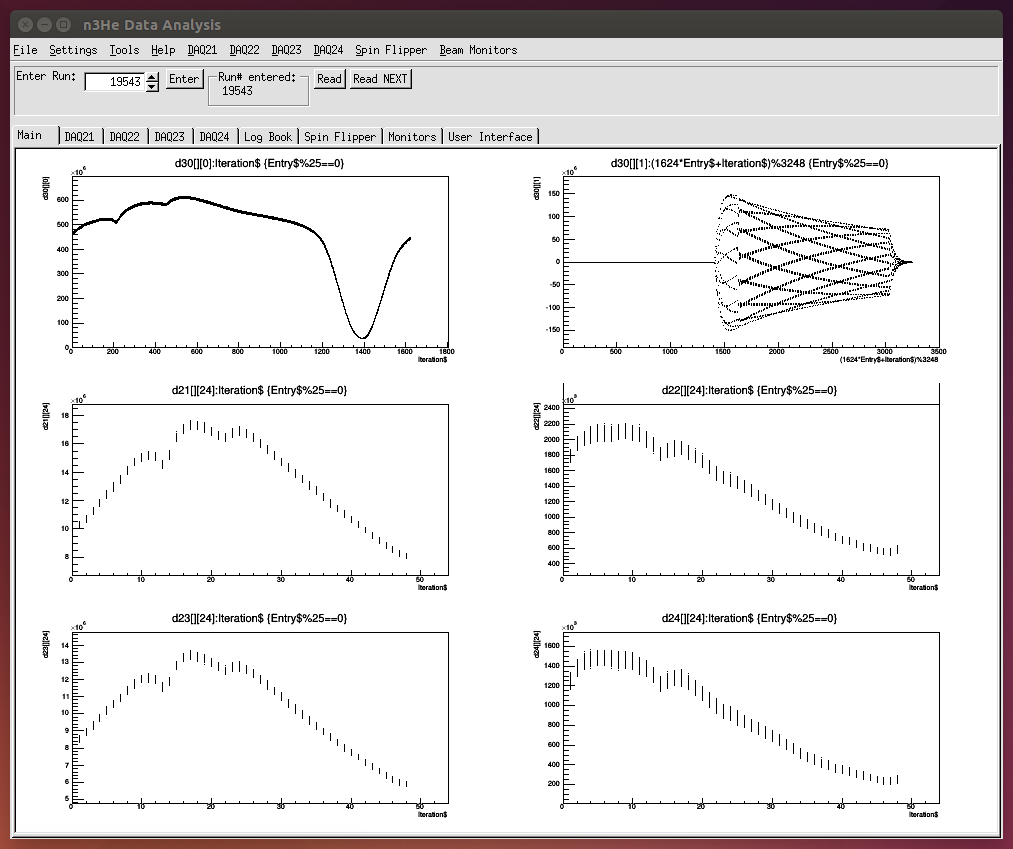
\includegraphics[width=6in]{data_browser.png}\\
\caption{The n3He data browser}\label{f2}
\end{figure}

\noindent
{\color{red} \rule{\linewidth}{1mm} }
 
\newpage
\section{Current tree structure in n3He analysis libary}

Currently n3He Tree has five branches corresponding to four clean DAQ and one dirty DAQ, following is the leaf list in the n3He Tree. 
\begin{lstlisting}
 DAQ21_LEAF "h21[48]/I:d21[49][48]/I"
 DAQ22_LEAF "h22[48]/I:d22[49][48]/I"
 DAQ23_LEAF "h23[48]/I:d23[49][48]/I"
 DAQ24_LEAF "h24[48]/I:d24[49][48]/I"
 DAQ30_LEAF "h30[2]/I:d30[1624][2]/I"
\end{lstlisting}
where h used to indicate header and d used to indicate detector signal. 21 to 24 are clean DAQs and 30 is dirty DAQ.

\begin{figure}[htb]
\centering
% Requires \usepackage{graphicx}
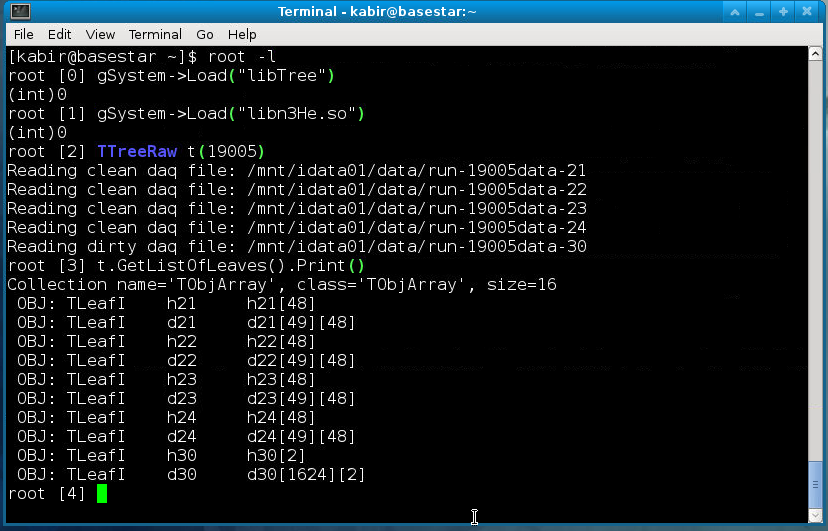
\includegraphics[width=6in]{treeStructure1.png}\\
\caption{The n3He leaf list}\label{f3}
\end{figure}

Now the library always skips the first four or five events since those might NOT be reliable. As a result the number of events in any branch for a typical n3He run is 24996 or 24995(This offset is set dynamically).

\begin{figure}[htb]
\centering
% Requires \usepackage{graphicx}
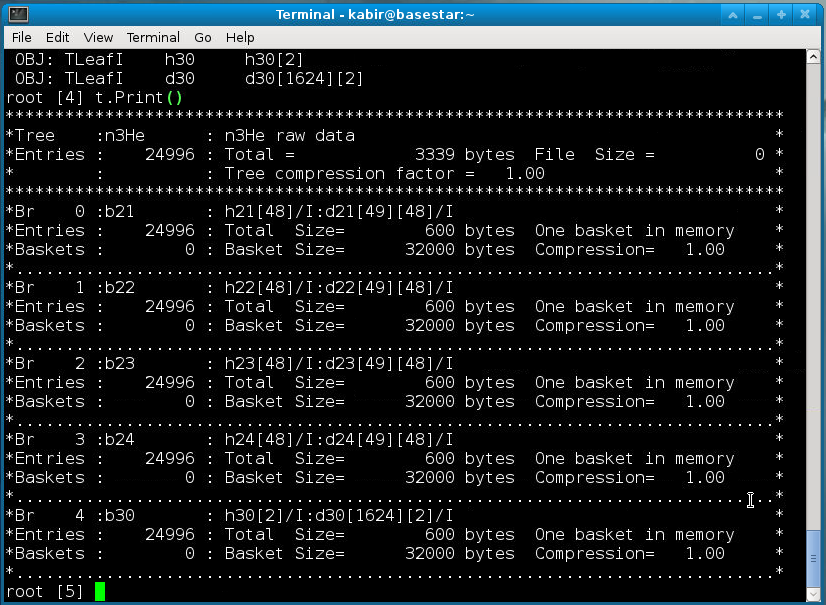
\includegraphics[width=6in]{treeStructure2.png}\\
\caption{The n3He tree structure}\label{f4}
\end{figure}

\noindent
{\color{red} \rule{\linewidth}{1mm} }
 
\newpage
\section{Sample analysis}
Sample online analysis on basestar:
\begin{lstlisting}
//OnlineAnalysis.C
//Demo Online Analysis using n3He Library.(By Online I mean  'from CINT, doing analysis on the fly, less thoughtful but preferred by in some conditions')
//Author: Latiful Kabir
//Date: 12/23/14

void OnlineAnalysis()
{
    gSystem->Load("libTree");    //You need to load libTree first in order to Load libn3He. This is not necessary if you include TTree.h
    gSystem->Load("libn3He.so");

    TTreeRaw *t=new TTreeRaw(19900);
    t->Draw("d21[][0]:Iteration$");
}

\end{lstlisting}

This script when you run using \textcolor{magenta}{root -l OnlineAnalysis.C} will produce the following output:

\begin{figure}[htb]
\centering
% Requires \usepackage{graphicx}
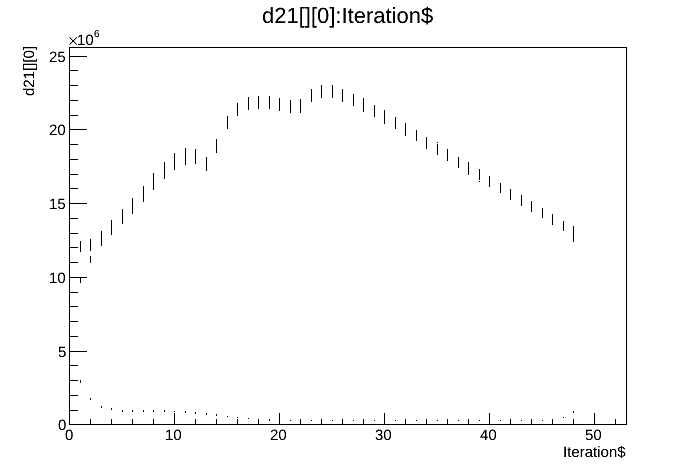
\includegraphics[width=6in]{OnlineAnalysis.png}\\
\caption{The Output from OnlineAnalysis.C}\label{f5}
\end{figure}

\newpage
Sample offline analysis on basestar:
\begin{lstlisting}
//OfflineAnalysis.C
//Demo Offline Analysis using n3He Library.(By Offline I mean  'in a script more thoughtful and serious analysis unlike from CINT)
//This script shows how to accress Tree using SetAddress
// and plots only the all event/pulses of channel-0
//Author: Latiful Kabir
//Date: 01/14/15
//This is the fastest and most preferred method for reading Tree 

#include<TTree.h>
#include<TBranch.h>
#include<TGraph.h>

void OfflineAnalysis(){

    //Load the library unless loaded automatically by ROOT
     gSystem->Load("libTree");
     gSystem->Load("libn3He.so");
 
  //Create a TTreeRaw object with desired run number
  TTreeRaw *t=new TTreeRaw(17900);
  t->Print();  // Print to see what's inside the Tree
  int ch=0; //Channel to analyze

  //Create a struc buffer to keep your events 
  struct myData
  {
      int header[48];
      int det[49][48];  
  };

  myData md;
  
  //Get the branch you want to analyze
  TBranch *b=t->GetBranch("b21");
  b->SetAddress(&md.header[ch]);

//--------------------------------------------------

  TGraph *g=new TGraph();

  //Loop through all the events in the run.
  for(int i = 0;i < b->GetEntries();i++)
  {
      //Load the samples for a event/pulse in buffer
      b->GetEntry(i);

      //Loops through the sample for the loaded event
      for(int k=0;k<49;k++)
 	  g->SetPoint(i*49+k,i*49+k,md.det[k][ch]);
  }

  g->Draw("AP");
  delete t;
}
\end{lstlisting}
This script when you run using \textcolor{magenta}{root -l OfflineAnalysis.C} will produce the following output when zoomed in:

\begin{figure}[htb]
\centering
% Requires \usepackage{graphicx}
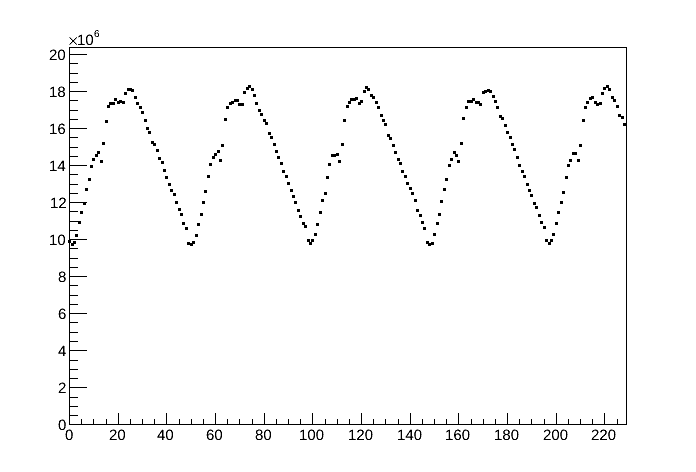
\includegraphics[width=6in]{OfflineAnalysis.png}\\
\caption{The output from OfflineAnalysis.C}\label{f6}
\end{figure}

\noindent
{\color{red} \rule{\linewidth}{1mm} }
 
\newpage
\section{Reference for TTreeRaw class}
The base Classis  TTree.\\
As a result all data and member functions from TTree are automatically inherited. For a list of TTree data and member functions go \href{https://root.cern.ch/root/html/TTree.html}{here}
\begin{lstlisting}
public:

   TString dataPath;
   TString *DaqLeaf;
   TString *dataFile;
   static int module[5];

   TBranch *b21,*b22,*b23,*b24,*b30;

     TTreeRaw(int runNumber);
    ~TTreeRaw();

\end{lstlisting}

This list will be updated gradually as new functionality is added to the TTreeRaw class.

\noindent
{\color{red} \rule{\linewidth}{1mm} }
 
\end{document}
